% ============================================================================
% October 9, 2026 build (agent draft). Copy of 02c_motivating_evidence.tex
% brought in line with the JMP deck of Oct 9 (latex/JMP_slides/JMP_slides.tex):
% the deck motivates the model with three channels (tenure segmentation,
% wealth and down payments, the intergenerational allocation of large homes)
% and no longer shows the CPS fertility-by-income table, so that subsection
% is cut here. The moving-reasons panels are the deck's appendix figures
% (JMP_slides/assets/mv_*_f_c_y_all.png, PSID, May event-study estimates).
% Register: Boar, Gorea and Midrigan, Section 2.
% ============================================================================
\providecommand{\mocktodo}[1]{\textcolor{red}{[TODO: #1]}}

\section{Motivating Evidence}
\label{sec:empirical-evidence}

This section documents three facts that shape the model. First, large homes
are mostly owned: the rental market offers few dwellings large enough for a
family with several children. Second, most large owner-occupied homes are held
by older households without children at home, while young families hold few.
Third, households enlarge their dwelling and move into ownership within a few
years of the first birth, and then move less. Together these facts describe
how a young family obtains space for children. It needs a larger home early
in adult life, when its savings are smallest, and the large homes are mostly
sold rather than rented and mostly held by an older generation. Space,
tenure and wealth are therefore linked at the moment fertility is decided.
None of the facts isolates an exogenous change in fertility, and I do not use
them to argue that housing costs lower fertility.
Appendix~\ref{app:empirical-data} describes the data.

\subsection{Large homes are owned}

Figure~\ref{fig:tenure-by-size} divides the homes of each size in the 2023
American Housing Survey (AHS) by tenure. Of the homes with four or more
bedrooms, 87 percent are owner-occupied and 9 percent are rented; of the homes
with at most one bedroom, 13 percent are owner-occupied and 74 percent are
rented. Measured in rooms, the unit used in the rest of the paper, 43.0
percent of owner-occupied homes have seven or more rooms, against 7.5 percent
of rented homes. The gap persists among families: in households with children,
owners occupy 6.8 rooms on average and renters 5.2. Nearly half of renter households
with children, 48.7 percent, live in homes with at most two bedrooms,
against 7.4 percent of owner households with children.
% [DATA] AHS 2023 ahs_children_space_mismatch.csv (code/data/ahs_supply_snapshot/
% output_ahs_family_unit_menu_national/). These shares describe the
homes households occupy, not the homes offered for rent. They show that, in
the existing stock, a family that wants a large dwelling typically buys one.
% [DATA] AHS 2023 national PUF; code/data/ahs_supply_snapshot/ (sandbox
% FIGURES.md maps the figure to its source).

\begin{figure}[t]
\centering
\includegraphics[width=0.62\linewidth]{ahs_tenure_share_within_size}
\caption{Tenure of the housing stock by number of bedrooms (AHS 2023)}
\label{fig:tenure-by-size}
\par\smallskip
\begin{minipage}{0.92\linewidth}
\footnotesize\textit{Notes:} Each bar divides the housing units with the
stated number of bedrooms into owner-occupied units, units rented for cash,
and vacant units. Units occupied without payment of cash rent and units whose
occupants have a usual residence elsewhere are excluded. Weighted by the
housing-unit weight. Source: American Housing Survey 2023, national
public-use file.
\end{minipage}
\end{figure}

\subsection{Who holds the large homes}

Most large owner-occupied homes are held by households without children at
home, and the largest group among them is old. Figure~\ref{fig:large-homes}
divides the owner-occupied homes with six or more rooms in 42 large
metropolitan areas in the 2023 American Community Survey (ACS) among six groups
of households, defined by the age of the householder and by whether a child of
the householder younger than 18 lives in the home. Households aged 60 to 85
without children at home hold 40.0 percent of these homes, and households
aged 40 to 59 without children at home another 21.8 percent. Households aged
22 to 39 with children hold 10.6 percent. Across all ages, 68.3 percent of the
large owner-occupied homes house no child of the householder, close to the
72.9 percent of all households in these areas without a child at home. What
the figure shows is therefore where the large homes sit by age, not that
childless households hold more than their share. I call the concentration of
large owner-occupied homes among older households the intergenerational
allocation of housing. The figure does not show that older households would
sell at some price, or that young families would have more children if they
held these homes.
% [DATA] ACS 2023 one-year, 42 metros, householders 22-85, 289,109 households;
% numbers as in the Oct 4 sandbox paper (reviewed there).
\mocktodo{name the builder of the large-homes figure in the data appendix
(not found in code/ by the Oct 4 sandbox review); the sandbox calls this
"intergenerational misallocation", which the title uses; choose the term.}

\begin{figure}[t]
\centering
\includegraphics[width=0.9\linewidth]{large_homes_by_age_children_acs2023}
\caption{Who holds the large owner-occupied homes (ACS 2023)}
\label{fig:large-homes}
\par\smallskip
\begin{minipage}{0.92\linewidth}
\footnotesize\textit{Notes:} Each bar is the share of owner-occupied homes
with six or more rooms held by households in the group; the six shares sum to
100 percent. Groups are defined by the age of the householder and by whether
an own child of the householder younger than 18 lives in the household.
Householders aged 22 to 85 in 42 large metropolitan areas, weighted by the
household weight; 289,109 households.
\end{minipage}
\end{figure}

\subsection{Housing around the first birth}

The Panel Study of Income Dynamics (PSID) follows the same families from 1968
to 2019. I date each woman's first birth from her full history of biological
children and estimate event studies of her household's housing around it,
comparing first-time mothers with women who never have children, with the
estimator of Sun and Abraham (2021) and person and year
fixed effects. The reference window is two to three years before the birth,
so that moves made while expecting a child count as responses. The sample
keeps one woman per household and year who is its reference person or spouse.
% [DATA] mock 02_empirical_evidence.tex and data_appendix.tex; 63,338
% person-years, 3,655 first-time mothers, 1,654 childless women.

Households add about one room within four years of the first birth.
Figure~\ref{fig:emp-rooms-path} reports the path. The dwelling is 0.41 rooms
larger than in the reference window in the year of the birth, 0.82 rooms one
to two years later, and 1.03 rooms (standard error 0.07) three to four years
after it, on a base of 4.7 rooms. Fixing household position before the birth,
which removes a pre-trend that reflects who heads a household, the increase at
three to four years is 1.47 rooms (0.05). The added space comes with a move
into ownership, after which families move less (Figure~\ref{fig:emp-tenure-moves}).
The ownership rate is 11 percentage points higher in the birth window and 16
points higher three to four years later, on a base of 41 percent. The
probability of having moved since the previous interview falls by 16 to 21
points after the birth and stays lower for a decade, and among those who do
move, the share moving for more space doubles, from 12 to about 25 percent.
The ACS shows the same pattern at a point in time: among household heads aged
30 to 55, those whose oldest child is under four are 12.8 percentage points
more likely to own than heads without children.
% [DATA] ACS 2005-06 recent-parent gap 0.12761 (same as Section 4 target).

\begin{figure}[t]
\centering
\includegraphics[width=0.88\linewidth]{first_birth_rooms_psid}
\caption{Rooms around the first birth (PSID)}
\label{fig:emp-rooms-path}
\par\smallskip
\begin{minipage}{0.92\linewidth}
\footnotesize\textit{Notes:} Interaction-weighted event-study estimates in
two-year windows of event time, with 95 percent confidence intervals from
standard errors clustered by person. One woman per household-year who is the
reference person or spouse; 63,338 person-years, 3,655 first-time parents and
1,654 childless women. The hollow marker is the omitted reference window,
years $-3$ and $-2$. Mean rooms in the reference window: 4.70.
\end{minipage}
\end{figure}

\begin{figure}[t]
\centering
\includegraphics[width=0.92\linewidth]{first_birth_tenure_moves_psid}
\caption{Ownership and moving around the first birth (PSID)}
\label{fig:emp-tenure-moves}
\par\smallskip
\begin{minipage}{0.92\linewidth}
\footnotesize\textit{Notes:} Same sample, estimator and reference window as
Figure~\ref{fig:emp-rooms-path}. ``Moved for more space'' equals one if the
household moved since the previous interview and gave more space as the first
reason. Means in the reference window: ownership 0.41, moved 0.58.
\end{minipage}
\end{figure}

Figure~\ref{fig:emp-move-reasons} splits moves by the reason the household
gives. The annual probability of moving for more or better housing rises by
about 2.5 percentage points in the year before and the year of the birth and
returns to its earlier level within about five years. Moves for the
neighborhood, schools or proximity do not change around the birth. The
response to the first child is a demand for space, not for location.

\begin{figure}[t]
\centering
\begin{minipage}{0.48\linewidth}\centering
{\small Expansion or better housing}\par\smallskip
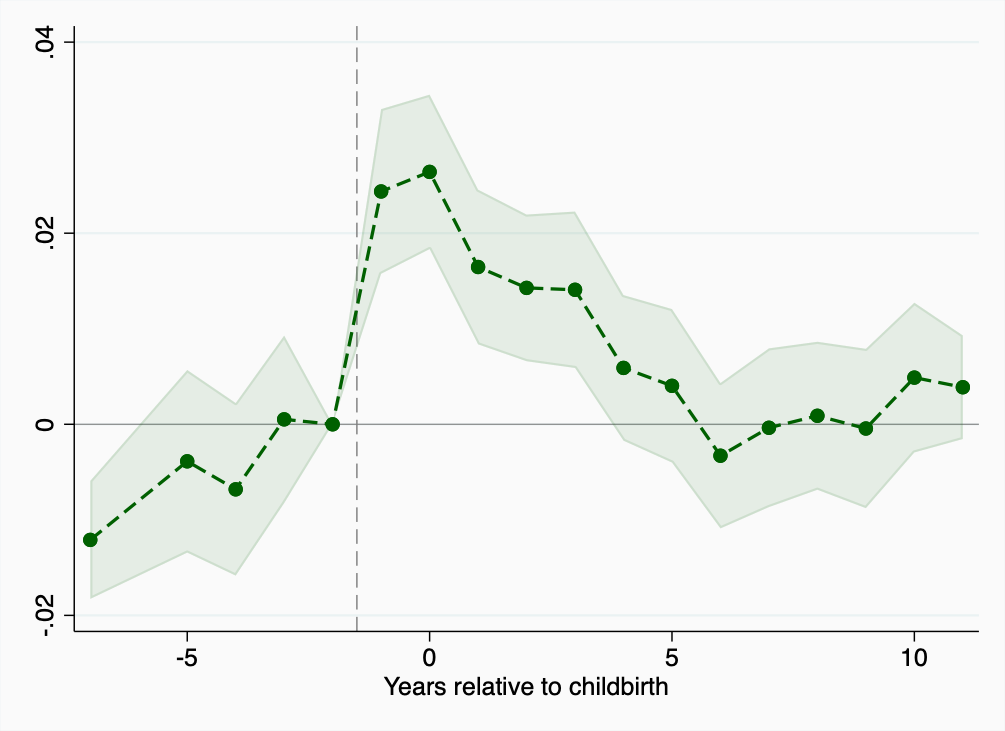
\includegraphics[width=\linewidth]{../JMP_slides/assets/mv_s_f_c_y_all.png}
\end{minipage}\hfill
\begin{minipage}{0.48\linewidth}\centering
{\small Neighborhood, schools, or proximity}\par\smallskip
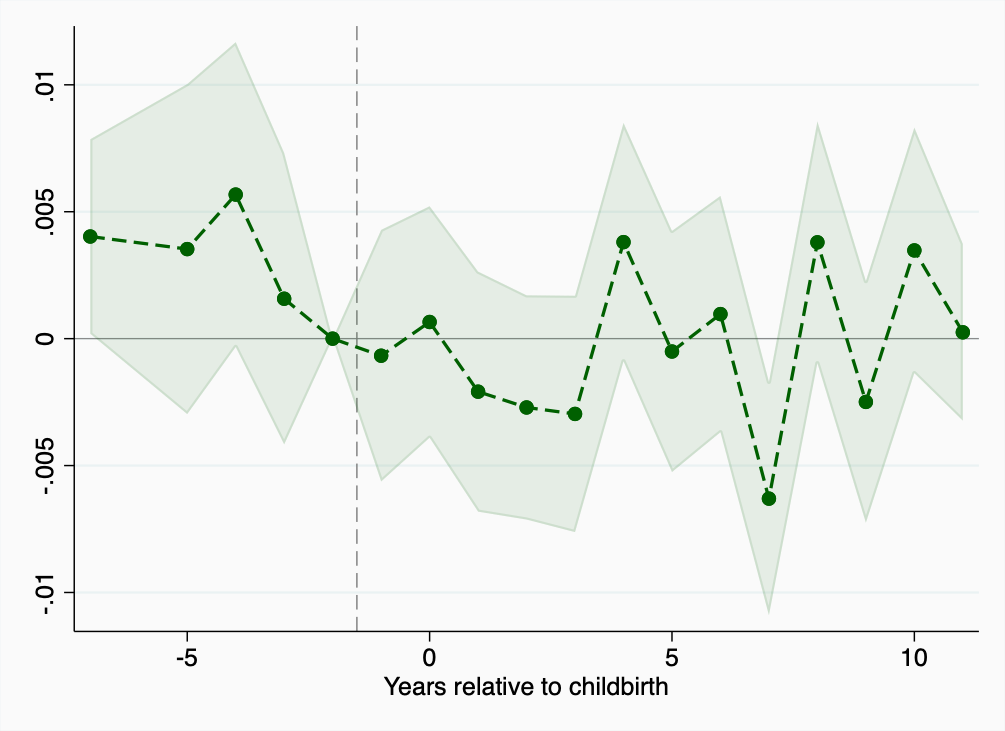
\includegraphics[width=\linewidth]{../JMP_slides/assets/mv_n_f_c_y_all.png}
\end{minipage}
\caption{Reasons for moving around the first birth (PSID)}
\label{fig:emp-move-reasons}
\par\smallskip
\begin{minipage}{0.92\linewidth}
\footnotesize\textit{Notes:} Event-study estimates of the probability of a move
for the stated reason, relative to the reference window, from the May
specification of the PSID event study.
\mocktodo{these are the deck's May estimates; the rooms and tenure figures
above are the September estimates. Re-estimate the reasons on the September
sample, or say in the notes that they come from the earlier specification.}
\end{minipage}
\end{figure}

\subsection{Implications for the model}

These facts motivate the three features that set the model apart from a
life-cycle model with a generic cost of children. Because children need
space and households add it around the first birth, fertility and housing
are chosen jointly, and a family needs a minimum of space before additional
rooms raise its welfare. Because large homes are mostly owned, the model
limits the size of rental units, so a family that wants a large home must buy
it; I call this tenure segmentation. Because buying requires a down payment,
paid out of wealth and current income, the wealth of young households and its
timing matter.
And because the large homes sit with older households, the price of space for
young families depends on the whole age distribution of households; the model
is an overlapping-generations economy in which one house price clears a
market shared by all ages.
